
% ------------------------------------- FIG
\begin{figure}
% GNUPLOT: LaTeX picture with Postscript
\begingroup
  \makeatletter
  \providecommand\color[2][]{%
    \GenericError{(gnuplot) \space\space\space\@spaces}{%
      Package color not loaded in conjunction with
      terminal option `colourtext'%
    }{See the gnuplot documentation for explanation.%
    }{Either use 'blacktext' in gnuplot or load the package
      color.sty in LaTeX.}%
    \renewcommand\color[2][]{}%
  }%
  \providecommand\includegraphics[2][]{%
    \GenericError{(gnuplot) \space\space\space\@spaces}{%
      Package graphicx or graphics not loaded%
    }{See the gnuplot documentation for explanation.%
    }{The gnuplot epslatex terminal needs graphicx.sty or graphics.sty.}%
    \renewcommand\includegraphics[2][]{}%
  }%
  \providecommand\rotatebox[2]{#2}%
  \@ifundefined{ifGPcolor}{%
    \newif\ifGPcolor
    \GPcolorfalse
  }{}%
  \@ifundefined{ifGPblacktext}{%
    \newif\ifGPblacktext
    \GPblacktexttrue
  }{}%
  % define a \g@addto@macro without @ in the name:
  \let\gplgaddtomacro\g@addto@macro
  % define empty templates for all commands taking text:
  \gdef\gplbacktext{}%
  \gdef\gplfronttext{}%
  \makeatother
  \ifGPblacktext
    % no textcolor at all
    \def\colorrgb#1{}%
    \def\colorgray#1{}%
  \else
    % gray or color?
    \ifGPcolor
      \def\colorrgb#1{\color[rgb]{#1}}%
      \def\colorgray#1{\color[gray]{#1}}%
      \expandafter\def\csname LTw\endcsname{\color{white}}%
      \expandafter\def\csname LTb\endcsname{\color{black}}%
      \expandafter\def\csname LTa\endcsname{\color{black}}%
      \expandafter\def\csname LT0\endcsname{\color[rgb]{1,0,0}}%
      \expandafter\def\csname LT1\endcsname{\color[rgb]{0,1,0}}%
      \expandafter\def\csname LT2\endcsname{\color[rgb]{0,0,1}}%
      \expandafter\def\csname LT3\endcsname{\color[rgb]{1,0,1}}%
      \expandafter\def\csname LT4\endcsname{\color[rgb]{0,1,1}}%
      \expandafter\def\csname LT5\endcsname{\color[rgb]{1,1,0}}%
      \expandafter\def\csname LT6\endcsname{\color[rgb]{0,0,0}}%
      \expandafter\def\csname LT7\endcsname{\color[rgb]{1,0.3,0}}%
      \expandafter\def\csname LT8\endcsname{\color[rgb]{0.5,0.5,0.5}}%
    \else
      % gray
      \def\colorrgb#1{\color{black}}%
      \def\colorgray#1{\color[gray]{#1}}%
      \expandafter\def\csname LTw\endcsname{\color{white}}%
      \expandafter\def\csname LTb\endcsname{\color{black}}%
      \expandafter\def\csname LTa\endcsname{\color{black}}%
      \expandafter\def\csname LT0\endcsname{\color{black}}%
      \expandafter\def\csname LT1\endcsname{\color{black}}%
      \expandafter\def\csname LT2\endcsname{\color{black}}%
      \expandafter\def\csname LT3\endcsname{\color{black}}%
      \expandafter\def\csname LT4\endcsname{\color{black}}%
      \expandafter\def\csname LT5\endcsname{\color{black}}%
      \expandafter\def\csname LT6\endcsname{\color{black}}%
      \expandafter\def\csname LT7\endcsname{\color{black}}%
      \expandafter\def\csname LT8\endcsname{\color{black}}%
    \fi
  \fi
  \setlength{\unitlength}{0.0500bp}%
  \begin{picture}(5040.00,3600.00)%
    \gplgaddtomacro\gplbacktext{%
      \csname LTb\endcsname%
      \put(472,360){\makebox(0,0)[r]{\strut{}}}%
      \put(472,623){\makebox(0,0)[r]{\strut{}400}}%
      \put(472,827){\makebox(0,0)[r]{\strut{}}}%
      \put(472,994){\makebox(0,0)[r]{\strut{}}}%
      \put(472,1134){\makebox(0,0)[r]{\strut{}}}%
      \put(472,1256){\makebox(0,0)[r]{\strut{}800}}%
      \put(472,1364){\makebox(0,0)[r]{\strut{}}}%
      \put(472,1460){\makebox(0,0)[r]{\strut{}1000}}%
      \put(472,2094){\makebox(0,0)[r]{\strut{}2000}}%
      \put(472,2465){\makebox(0,0)[r]{\strut{}}}%
      \put(472,2728){\makebox(0,0)[r]{\strut{}4000}}%
      \put(472,2931){\makebox(0,0)[r]{\strut{}}}%
      \put(472,3098){\makebox(0,0)[r]{\strut{}}}%
      \put(472,3239){\makebox(0,0)[r]{\strut{}}}%
      \put(788,140){\makebox(0,0){\strut{}}}%
      \put(2002,140){\makebox(0,0){\strut{}}}%
      \put(2712,140){\makebox(0,0){\strut{}}}%
      \put(3215,140){\makebox(0,0){\strut{}}}%
      \put(3606,140){\makebox(0,0){\strut{}}}%
      \put(3925,140){\makebox(0,0){\strut{}}}%
      \put(4195,140){\makebox(0,0){\strut{}}}%
      \put(4429,140){\makebox(0,0){\strut{}}}%
      \put(-100,1799){\rotatebox{-270}{\makebox(0,0){\strut{}runtime (ms)}}}%
      \put(2569,3569){\makebox(0,0){\strut{}Laplace on 2xQuad Core 2.0GHz Intel Harpertown}}%
      \put(788,2835){\rotatebox{-27}{\makebox(0,0)[l]{\strut{}Safe Get}}}%
      \put(788,2552){\rotatebox{-26.5}{\makebox(0,0)[l]{\strut{}Unsafe Get}}}%
      \put(788,1935){\rotatebox{-16.5}{\makebox(0,0)[l]{\strut{}Unsafe Unrolled Get}}}%
      \put(788,1312){\rotatebox{-6}{\makebox(0,0)[l]{\strut{}Safe Unrolled Stencil}}}%
      \put(788,689){\makebox(0,0)[l]{\strut{}Handwritten C with GCC 4.4.3}}%
    }%
    \gplgaddtomacro\gplfronttext{%
    }%
    \gplbacktext
    \put(0,0){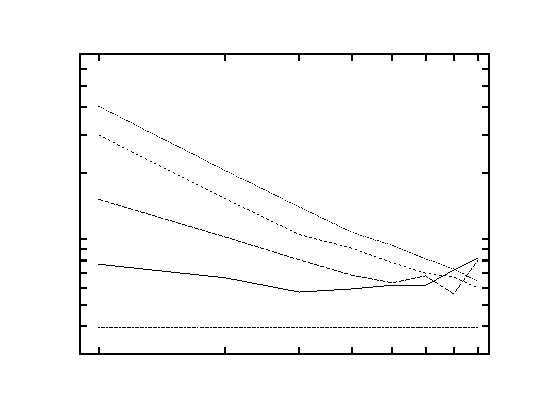
\includegraphics{data/laplace/tesla}}%
    \gplfronttext
  \end{picture}%
\endgroup
\vspace{-2.5em}
% GNUPLOT: LaTeX picture with Postscript
\begingroup
  \makeatletter
  \providecommand\color[2][]{%
    \GenericError{(gnuplot) \space\space\space\@spaces}{%
      Package color not loaded in conjunction with
      terminal option `colourtext'%
    }{See the gnuplot documentation for explanation.%
    }{Either use 'blacktext' in gnuplot or load the package
      color.sty in LaTeX.}%
    \renewcommand\color[2][]{}%
  }%
  \providecommand\includegraphics[2][]{%
    \GenericError{(gnuplot) \space\space\space\@spaces}{%
      Package graphicx or graphics not loaded%
    }{See the gnuplot documentation for explanation.%
    }{The gnuplot epslatex terminal needs graphicx.sty or graphics.sty.}%
    \renewcommand\includegraphics[2][]{}%
  }%
  \providecommand\rotatebox[2]{#2}%
  \@ifundefined{ifGPcolor}{%
    \newif\ifGPcolor
    \GPcolorfalse
  }{}%
  \@ifundefined{ifGPblacktext}{%
    \newif\ifGPblacktext
    \GPblacktexttrue
  }{}%
  % define a \g@addto@macro without @ in the name:
  \let\gplgaddtomacro\g@addto@macro
  % define empty templates for all commands taking text:
  \gdef\gplbacktext{}%
  \gdef\gplfronttext{}%
  \makeatother
  \ifGPblacktext
    % no textcolor at all
    \def\colorrgb#1{}%
    \def\colorgray#1{}%
  \else
    % gray or color?
    \ifGPcolor
      \def\colorrgb#1{\color[rgb]{#1}}%
      \def\colorgray#1{\color[gray]{#1}}%
      \expandafter\def\csname LTw\endcsname{\color{white}}%
      \expandafter\def\csname LTb\endcsname{\color{black}}%
      \expandafter\def\csname LTa\endcsname{\color{black}}%
      \expandafter\def\csname LT0\endcsname{\color[rgb]{1,0,0}}%
      \expandafter\def\csname LT1\endcsname{\color[rgb]{0,1,0}}%
      \expandafter\def\csname LT2\endcsname{\color[rgb]{0,0,1}}%
      \expandafter\def\csname LT3\endcsname{\color[rgb]{1,0,1}}%
      \expandafter\def\csname LT4\endcsname{\color[rgb]{0,1,1}}%
      \expandafter\def\csname LT5\endcsname{\color[rgb]{1,1,0}}%
      \expandafter\def\csname LT6\endcsname{\color[rgb]{0,0,0}}%
      \expandafter\def\csname LT7\endcsname{\color[rgb]{1,0.3,0}}%
      \expandafter\def\csname LT8\endcsname{\color[rgb]{0.5,0.5,0.5}}%
    \else
      % gray
      \def\colorrgb#1{\color{black}}%
      \def\colorgray#1{\color[gray]{#1}}%
      \expandafter\def\csname LTw\endcsname{\color{white}}%
      \expandafter\def\csname LTb\endcsname{\color{black}}%
      \expandafter\def\csname LTa\endcsname{\color{black}}%
      \expandafter\def\csname LT0\endcsname{\color{black}}%
      \expandafter\def\csname LT1\endcsname{\color{black}}%
      \expandafter\def\csname LT2\endcsname{\color{black}}%
      \expandafter\def\csname LT3\endcsname{\color{black}}%
      \expandafter\def\csname LT4\endcsname{\color{black}}%
      \expandafter\def\csname LT5\endcsname{\color{black}}%
      \expandafter\def\csname LT6\endcsname{\color{black}}%
      \expandafter\def\csname LT7\endcsname{\color{black}}%
      \expandafter\def\csname LT8\endcsname{\color{black}}%
    \fi
  \fi
  \setlength{\unitlength}{0.0500bp}%
  \begin{picture}(5040.00,2160.00)%
    \gplgaddtomacro\gplbacktext{%
      \csname LTb\endcsname%
      \put(472,335){\makebox(0,0)[r]{\strut{} 1}}%
      \put(472,842){\makebox(0,0)[r]{\strut{} 2}}%
      \put(472,1350){\makebox(0,0)[r]{\strut{} 4}}%
      \put(472,1857){\makebox(0,0)[r]{\strut{} 8}}%
      \put(788,-4){\makebox(0,0){\strut{} 1}}%
      \put(2002,-4){\makebox(0,0){\strut{} 2}}%
      \put(2712,-4){\makebox(0,0){\strut{} 3}}%
      \put(3215,-4){\makebox(0,0){\strut{} 4}}%
      \put(3606,-4){\makebox(0,0){\strut{} 5}}%
      \put(3925,-4){\makebox(0,0){\strut{} 6}}%
      \put(4195,-4){\makebox(0,0){\strut{} 7}}%
      \put(4429,-4){\makebox(0,0){\strut{} 8}}%
      \put(100,1079){\rotatebox{-270}{\makebox(0,0){\strut{}speedup}}}%
      \put(2569,-334){\makebox(0,0){\strut{}threads (on 8 PEs)}}%
    }%
    \gplgaddtomacro\gplfronttext{%
    }%
    \gplbacktext
    \put(0,0){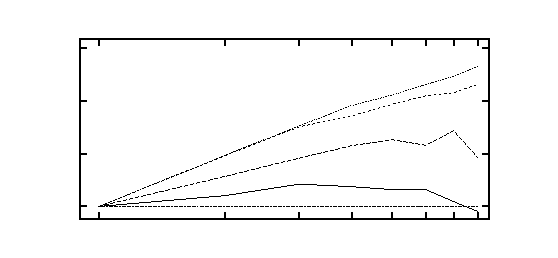
\includegraphics{data/laplace/tesla-speedup}}%
    \gplfronttext
  \end{picture}%
\endgroup

\vspace{2em}
\caption{Laplace relaxation 300x300 image, 1000 iterations}
\label{fig:LaplaceBenchmarks}
\end{figure}


\section{Benchmarks}

In this section we discuss the performance of our stencil benchmarks. All measurements were taken on a 2GHz 2xQuadCore Intel E5405 Harpertown server which has 6MB of L2 cache per processor and no hardware threading.


% -----------------------------------------------------------------------------
\subsection{Laplace Again} 
Figure \ref{fig:LaplaceBenchmarks} shows the performance of our Laplace benchmark. The Safe Get version uses the code from Figure \ref{fig:LaplaceIndex} with bounds checked indexing, while Unsafe Get is the same code with unchecked indexing. Unsafe Unrolled Get is the bounds checked version, but using the unrolled filling function in Figure \ref{fig:BlockEvaluation}. Safe Unrolled Stencil uses the unrolled filling function, as well as our cursored arrays. The single threaded Handwritten C version is about 45\% faster than our best Haskell result, which is achieved with 3 threads. The C version beats the Haskell one because it doesn't need the initial @x + y * width@ calculations corresponding to the application of @make@ in Figure \ref{fig:BlockEvaluation}, and there isn't enough sharing inherent in the Laplace stencil for the Haskell version to exploit. For this, note the small amount of overlap in four Laplace stencils placed side-by-side. Still, it's not an unreasonable result for a Haskell program, considering that the C version produces an inner loop that appears close to optimal. We tried eliminating the application of @make@, but this turned out not to be an improvement due to the extra register required to maintain the centre index between loop iterations. 

Figure \ref{fig:LaplaceBenchmarks} also contains an important lesson for anyone interested in parallelism in functional languages. The least efficient version of our solver has best speedup graph, yet the most efficient one has the worst. To argue that a particular parallel computing system is useful, one cannot simply present the speedup vs number of cores, as this does not discount the possibility of large linear inefficiencies. In practice we have found the failure of unboxing or fusion on a given benchmark to cause in excess of a 10x linear slowdown, while maintaining a good speedup graph. 

For this benchmark we used an image size of 300x300, matching to our earlier work in \cite{Keller:repa}. In the end, it appears as though the speedup of this benchmark is limited by scheduling issues. Figure \ref{fig:LaplaceVariation} shows the huge variation in runtime for 100 consecutive runs using 4 threads. Increasing the efficiency of our inner loop has also reduced the grain size of the computation. When the grain size is small, there is a high chance that some threads will have started (or completed) their work before the others are scheduled by the OS. To fix this problem we expect that we need \emph{gang scheduling} \cite{Feitelson:gang-scheduling}, which ensures that all threads run in lockstep, instead of being independently scheduled whenever the OS ``feels like it''. 

\begin{figure}
% GNUPLOT: LaTeX picture with Postscript
\begingroup
  \makeatletter
  \providecommand\rotatebox[2]{#2}%
  \@ifundefined{ifGPcolor}{%
    \newif\ifGPcolor
    \GPcolorfalse
  }{}%
  \@ifundefined{ifGPblacktext}{%
    \newif\ifGPblacktext
    \GPblacktexttrue
  }{}%
  % define a \g@addto@macro without @ in the name:
  \let\gplgaddtomacro\g@addto@macro
  % define empty templates for all commands taking text:
  \gdef\gplbacktext{}%
  \gdef\gplfronttext{}%
  \makeatother
  \ifGPblacktext
    % no textcolor at all
    \def\colorrgb#1{}%
    \def\colorgray#1{}%
  \else
    % gray or color?
    \ifGPcolor
      \def\colorrgb#1{\color[rgb]{#1}}%
      \def\colorgray#1{\color[gray]{#1}}%
      \expandafter\def\csname LTw\endcsname{\color{white}}%
      \expandafter\def\csname LTb\endcsname{\color{black}}%
      \expandafter\def\csname LTa\endcsname{\color{black}}%
      \expandafter\def\csname LT0\endcsname{\color[rgb]{1,0,0}}%
      \expandafter\def\csname LT1\endcsname{\color[rgb]{0,1,0}}%
      \expandafter\def\csname LT2\endcsname{\color[rgb]{0,0,1}}%
      \expandafter\def\csname LT3\endcsname{\color[rgb]{1,0,1}}%
      \expandafter\def\csname LT4\endcsname{\color[rgb]{0,1,1}}%
      \expandafter\def\csname LT5\endcsname{\color[rgb]{1,1,0}}%
      \expandafter\def\csname LT6\endcsname{\color[rgb]{0,0,0}}%
      \expandafter\def\csname LT7\endcsname{\color[rgb]{1,0.3,0}}%
      \expandafter\def\csname LT8\endcsname{\color[rgb]{0.5,0.5,0.5}}%
    \else
      % gray
      \def\colorrgb#1{\color{black}}%
      \def\colorgray#1{\color[gray]{#1}}%
      \expandafter\def\csname LTw\endcsname{\color{white}}%
      \expandafter\def\csname LTb\endcsname{\color{black}}%
      \expandafter\def\csname LTa\endcsname{\color{black}}%
      \expandafter\def\csname LT0\endcsname{\color{black}}%
      \expandafter\def\csname LT1\endcsname{\color{black}}%
      \expandafter\def\csname LT2\endcsname{\color{black}}%
      \expandafter\def\csname LT3\endcsname{\color{black}}%
      \expandafter\def\csname LT4\endcsname{\color{black}}%
      \expandafter\def\csname LT5\endcsname{\color{black}}%
      \expandafter\def\csname LT6\endcsname{\color{black}}%
      \expandafter\def\csname LT7\endcsname{\color{black}}%
      \expandafter\def\csname LT8\endcsname{\color{black}}%
    \fi
  \fi
  \setlength{\unitlength}{0.0500bp}%
  \begin{picture}(5040.00,1872.00)%
    \gplgaddtomacro\gplbacktext{%
      \csname LTb\endcsname%
      \put(372,468){\makebox(0,0)[r]{\strut{} 0}}%
      \put(372,772){\makebox(0,0)[r]{\strut{} 5}}%
      \put(372,1076){\makebox(0,0)[r]{\strut{} 10}}%
      \put(372,1379){\makebox(0,0)[r]{\strut{} 15}}%
      \put(372,1683){\makebox(0,0)[r]{\strut{} 20}}%
      \put(504,280){\makebox(0,0){\strut{} 500}}%
      \put(1310,280){\makebox(0,0){\strut{} 550}}%
      \put(2116,280){\makebox(0,0){\strut{} 600}}%
      \put(2923,280){\makebox(0,0){\strut{} 650}}%
      \put(3729,280){\makebox(0,0){\strut{} 700}}%
      \put(4535,280){\makebox(0,0){\strut{} 750}}%
      \put(0,1075){\rotatebox{-270}{\makebox(0,0){\strut{}count}}}%
      \put(2519,70){\makebox(0,0){\strut{}runtime (ms)}}%
      \put(2439,1562){\makebox(0,0)[l]{\strut{}100 consecutive runs of}}%
      \put(2439,1342){\makebox(0,0)[l]{\strut{}Safe Unrolled Stencil solver}}%
      \put(2439,1122){\makebox(0,0)[l]{\strut{}using 4 threads on 8 PEs}}%
    }%
    \gplgaddtomacro\gplfronttext{%
    }%
    \gplbacktext
    \put(0,0){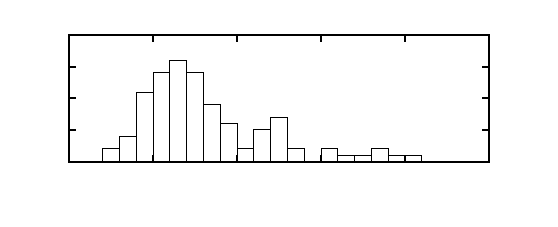
\includegraphics{data/laplace/tesla-repeat-qg-N4}}%
    \gplfronttext
  \end{picture}%
\endgroup

\caption{Variation in runtime of Unrolled Stencil Laplace}
\label{fig:LaplaceVariation}
\end{figure}



% -----------------------------------------------------------------------------
\subsection{Sobel Operator}
Figure \ref{fig:SobelAndCannyRuntime} shows the runtimes of the Sobel stencil applied to three image sizes. Also shown is a single threaded version using the @cv::Sobel@ function of OpenCV 2.2.0. This is using 32bit floats for the array values. To mitigate variance in runtime due to scheduling issues, we took the best result of 10 runs for each point. In this case, single threaded OpenCV is faster than our single threaded Haskell code primarily because it is using SSE SIMD intrinsics that we do not have access to from Haskell. The LLVM compiler also does not yet support auto-vectorisation to collect separate operations into fused SIMD instructions itself. With SSE, the OpenCV version is able to perform loads, stores, additions and multiplications on four packed 32bit floats at a time.  However, in all cases we are able to match OpenCV, with the larger image sizes only needing two threads to break even. 


% ------------------------------------- FIG
\begin{figure}
% GNUPLOT: LaTeX picture with Postscript
\begingroup
  \makeatletter
  \providecommand\color[2][]{%
    \GenericError{(gnuplot) \space\space\space\@spaces}{%
      Package color not loaded in conjunction with
      terminal option `colourtext'%
    }{See the gnuplot documentation for explanation.%
    }{Either use 'blacktext' in gnuplot or load the package
      color.sty in LaTeX.}%
    \renewcommand\color[2][]{}%
  }%
  \providecommand\includegraphics[2][]{%
    \GenericError{(gnuplot) \space\space\space\@spaces}{%
      Package graphicx or graphics not loaded%
    }{See the gnuplot documentation for explanation.%
    }{The gnuplot epslatex terminal needs graphicx.sty or graphics.sty.}%
    \renewcommand\includegraphics[2][]{}%
  }%
  \providecommand\rotatebox[2]{#2}%
  \@ifundefined{ifGPcolor}{%
    \newif\ifGPcolor
    \GPcolorfalse
  }{}%
  \@ifundefined{ifGPblacktext}{%
    \newif\ifGPblacktext
    \GPblacktexttrue
  }{}%
  % define a \g@addto@macro without @ in the name:
  \let\gplgaddtomacro\g@addto@macro
  % define empty templates for all commands taking text:
  \gdef\gplbacktext{}%
  \gdef\gplfronttext{}%
  \makeatother
  \ifGPblacktext
    % no textcolor at all
    \def\colorrgb#1{}%
    \def\colorgray#1{}%
  \else
    % gray or color?
    \ifGPcolor
      \def\colorrgb#1{\color[rgb]{#1}}%
      \def\colorgray#1{\color[gray]{#1}}%
      \expandafter\def\csname LTw\endcsname{\color{white}}%
      \expandafter\def\csname LTb\endcsname{\color{black}}%
      \expandafter\def\csname LTa\endcsname{\color{black}}%
      \expandafter\def\csname LT0\endcsname{\color[rgb]{1,0,0}}%
      \expandafter\def\csname LT1\endcsname{\color[rgb]{0,1,0}}%
      \expandafter\def\csname LT2\endcsname{\color[rgb]{0,0,1}}%
      \expandafter\def\csname LT3\endcsname{\color[rgb]{1,0,1}}%
      \expandafter\def\csname LT4\endcsname{\color[rgb]{0,1,1}}%
      \expandafter\def\csname LT5\endcsname{\color[rgb]{1,1,0}}%
      \expandafter\def\csname LT6\endcsname{\color[rgb]{0,0,0}}%
      \expandafter\def\csname LT7\endcsname{\color[rgb]{1,0.3,0}}%
      \expandafter\def\csname LT8\endcsname{\color[rgb]{0.5,0.5,0.5}}%
    \else
      % gray
      \def\colorrgb#1{\color{black}}%
      \def\colorgray#1{\color[gray]{#1}}%
      \expandafter\def\csname LTw\endcsname{\color{white}}%
      \expandafter\def\csname LTb\endcsname{\color{black}}%
      \expandafter\def\csname LTa\endcsname{\color{black}}%
      \expandafter\def\csname LT0\endcsname{\color{black}}%
      \expandafter\def\csname LT1\endcsname{\color{black}}%
      \expandafter\def\csname LT2\endcsname{\color{black}}%
      \expandafter\def\csname LT3\endcsname{\color{black}}%
      \expandafter\def\csname LT4\endcsname{\color{black}}%
      \expandafter\def\csname LT5\endcsname{\color{black}}%
      \expandafter\def\csname LT6\endcsname{\color{black}}%
      \expandafter\def\csname LT7\endcsname{\color{black}}%
      \expandafter\def\csname LT8\endcsname{\color{black}}%
    \fi
  \fi
  \setlength{\unitlength}{0.0500bp}%
  \begin{picture}(5040.00,3310.00)%
    \gplgaddtomacro\gplbacktext{%
      \csname LTb\endcsname%
      \put(472,496){\makebox(0,0)[r]{\strut{}}}%
      \put(472,638){\makebox(0,0)[r]{\strut{}}}%
      \put(472,759){\makebox(0,0)[r]{\strut{}}}%
      \put(472,863){\makebox(0,0)[r]{\strut{}800}}%
      \put(472,955){\makebox(0,0)[r]{\strut{}}}%
      \put(472,1037){\makebox(0,0)[r]{\strut{}1000}}%
      \put(472,1579){\makebox(0,0)[r]{\strut{}2000}}%
      \put(472,1895){\makebox(0,0)[r]{\strut{}}}%
      \put(472,2120){\makebox(0,0)[r]{\strut{}4000}}%
      \put(472,2294){\makebox(0,0)[r]{\strut{}}}%
      \put(472,2437){\makebox(0,0)[r]{\strut{}}}%
      \put(472,2557){\makebox(0,0)[r]{\strut{}}}%
      \put(472,2661){\makebox(0,0)[r]{\strut{}8000}}%
      \put(472,2753){\makebox(0,0)[r]{\strut{}}}%
      \put(472,2836){\makebox(0,0)[r]{\strut{}10000}}%
      \put(788,276){\makebox(0,0){\strut{} 1}}%
      \put(2002,276){\makebox(0,0){\strut{} 2}}%
      \put(2712,276){\makebox(0,0){\strut{} 3}}%
      \put(3215,276){\makebox(0,0){\strut{} 4}}%
      \put(3606,276){\makebox(0,0){\strut{} 5}}%
      \put(3925,276){\makebox(0,0){\strut{} 6}}%
      \put(4195,276){\makebox(0,0){\strut{} 7}}%
      \put(4429,276){\makebox(0,0){\strut{} 8}}%
      \put(-100,1737){\rotatebox{-270}{\makebox(0,0){\strut{}runtime (ms)}}}%
      \put(2569,0){\makebox(0,0){\strut{}threads (on 8 PEs)}}%
      \put(2569,3200){\makebox(0,0){\strut{}Canny on 2xQuad-core 2.0GHz Intel Harpertown}}%
      \put(3150,1841){\makebox(0,0)[l]{\strut{}1024x1024 image}}%
      \put(3215,1380){\makebox(0,0)[l]{\strut{} 768x768  image}}%
      \put(3215,792){\makebox(0,0)[l]{\strut{} 512x512  image}}%
    }%
    \gplgaddtomacro\gplfronttext{%
      \csname LTb\endcsname%
      \put(3630,2805){\makebox(0,0)[r]{\strut{}Safe Unrolled Stencil}}%
      \csname LTb\endcsname%
      \put(3630,2585){\makebox(0,0)[r]{\strut{}Single-threaded OpenCV}}%
    }%
    \gplbacktext
    \put(0,0){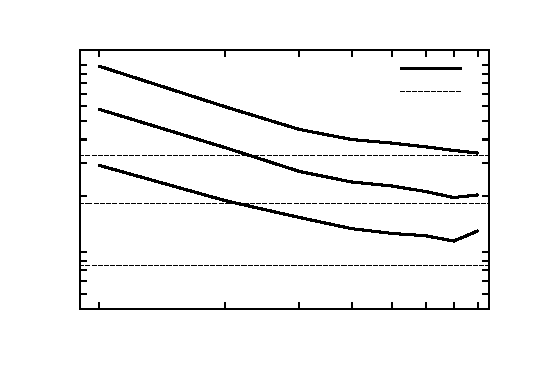
\includegraphics{data/canny/tesla-1024}}%
    \gplfronttext
  \end{picture}%
\endgroup

% GNUPLOT: LaTeX picture with Postscript
\begingroup
  \makeatletter
  \providecommand\color[2][]{%
    \GenericError{(gnuplot) \space\space\space\@spaces}{%
      Package color not loaded in conjunction with
      terminal option `colourtext'%
    }{See the gnuplot documentation for explanation.%
    }{Either use 'blacktext' in gnuplot or load the package
      color.sty in LaTeX.}%
    \renewcommand\color[2][]{}%
  }%
  \providecommand\includegraphics[2][]{%
    \GenericError{(gnuplot) \space\space\space\@spaces}{%
      Package graphicx or graphics not loaded%
    }{See the gnuplot documentation for explanation.%
    }{The gnuplot epslatex terminal needs graphicx.sty or graphics.sty.}%
    \renewcommand\includegraphics[2][]{}%
  }%
  \providecommand\rotatebox[2]{#2}%
  \@ifundefined{ifGPcolor}{%
    \newif\ifGPcolor
    \GPcolorfalse
  }{}%
  \@ifundefined{ifGPblacktext}{%
    \newif\ifGPblacktext
    \GPblacktexttrue
  }{}%
  % define a \g@addto@macro without @ in the name:
  \let\gplgaddtomacro\g@addto@macro
  % define empty templates for all commands taking text:
  \gdef\gplbacktext{}%
  \gdef\gplfronttext{}%
  \makeatother
  \ifGPblacktext
    % no textcolor at all
    \def\colorrgb#1{}%
    \def\colorgray#1{}%
  \else
    % gray or color?
    \ifGPcolor
      \def\colorrgb#1{\color[rgb]{#1}}%
      \def\colorgray#1{\color[gray]{#1}}%
      \expandafter\def\csname LTw\endcsname{\color{white}}%
      \expandafter\def\csname LTb\endcsname{\color{black}}%
      \expandafter\def\csname LTa\endcsname{\color{black}}%
      \expandafter\def\csname LT0\endcsname{\color[rgb]{1,0,0}}%
      \expandafter\def\csname LT1\endcsname{\color[rgb]{0,1,0}}%
      \expandafter\def\csname LT2\endcsname{\color[rgb]{0,0,1}}%
      \expandafter\def\csname LT3\endcsname{\color[rgb]{1,0,1}}%
      \expandafter\def\csname LT4\endcsname{\color[rgb]{0,1,1}}%
      \expandafter\def\csname LT5\endcsname{\color[rgb]{1,1,0}}%
      \expandafter\def\csname LT6\endcsname{\color[rgb]{0,0,0}}%
      \expandafter\def\csname LT7\endcsname{\color[rgb]{1,0.3,0}}%
      \expandafter\def\csname LT8\endcsname{\color[rgb]{0.5,0.5,0.5}}%
    \else
      % gray
      \def\colorrgb#1{\color{black}}%
      \def\colorgray#1{\color[gray]{#1}}%
      \expandafter\def\csname LTw\endcsname{\color{white}}%
      \expandafter\def\csname LTb\endcsname{\color{black}}%
      \expandafter\def\csname LTa\endcsname{\color{black}}%
      \expandafter\def\csname LT0\endcsname{\color{black}}%
      \expandafter\def\csname LT1\endcsname{\color{black}}%
      \expandafter\def\csname LT2\endcsname{\color{black}}%
      \expandafter\def\csname LT3\endcsname{\color{black}}%
      \expandafter\def\csname LT4\endcsname{\color{black}}%
      \expandafter\def\csname LT5\endcsname{\color{black}}%
      \expandafter\def\csname LT6\endcsname{\color{black}}%
      \expandafter\def\csname LT7\endcsname{\color{black}}%
      \expandafter\def\csname LT8\endcsname{\color{black}}%
    \fi
  \fi
  \setlength{\unitlength}{0.0500bp}%
  \begin{picture}(5040.00,3310.00)%
    \gplgaddtomacro\gplbacktext{%
      \csname LTb\endcsname%
      \put(472,496){\makebox(0,0)[r]{\strut{}}}%
      \put(472,638){\makebox(0,0)[r]{\strut{}}}%
      \put(472,759){\makebox(0,0)[r]{\strut{}}}%
      \put(472,863){\makebox(0,0)[r]{\strut{}800}}%
      \put(472,955){\makebox(0,0)[r]{\strut{}}}%
      \put(472,1037){\makebox(0,0)[r]{\strut{}1000}}%
      \put(472,1579){\makebox(0,0)[r]{\strut{}2000}}%
      \put(472,1895){\makebox(0,0)[r]{\strut{}}}%
      \put(472,2120){\makebox(0,0)[r]{\strut{}4000}}%
      \put(472,2294){\makebox(0,0)[r]{\strut{}}}%
      \put(472,2437){\makebox(0,0)[r]{\strut{}}}%
      \put(472,2557){\makebox(0,0)[r]{\strut{}}}%
      \put(472,2661){\makebox(0,0)[r]{\strut{}8000}}%
      \put(472,2753){\makebox(0,0)[r]{\strut{}}}%
      \put(472,2836){\makebox(0,0)[r]{\strut{}10000}}%
      \put(788,276){\makebox(0,0){\strut{} 1}}%
      \put(2002,276){\makebox(0,0){\strut{} 2}}%
      \put(2712,276){\makebox(0,0){\strut{} 3}}%
      \put(3215,276){\makebox(0,0){\strut{} 4}}%
      \put(3606,276){\makebox(0,0){\strut{} 5}}%
      \put(3925,276){\makebox(0,0){\strut{} 6}}%
      \put(4195,276){\makebox(0,0){\strut{} 7}}%
      \put(4429,276){\makebox(0,0){\strut{} 8}}%
      \put(-100,1737){\rotatebox{-270}{\makebox(0,0){\strut{}runtime (ms)}}}%
      \put(2569,0){\makebox(0,0){\strut{}threads (on 8 PEs)}}%
      \put(2569,3200){\makebox(0,0){\strut{}Canny on 2xQuad-core 2.0GHz Intel Harpertown}}%
      \put(3150,1841){\makebox(0,0)[l]{\strut{}1024x1024 image}}%
      \put(3215,1380){\makebox(0,0)[l]{\strut{} 768x768  image}}%
      \put(3215,792){\makebox(0,0)[l]{\strut{} 512x512  image}}%
    }%
    \gplgaddtomacro\gplfronttext{%
      \csname LTb\endcsname%
      \put(3630,2805){\makebox(0,0)[r]{\strut{}Safe Unrolled Stencil}}%
      \csname LTb\endcsname%
      \put(3630,2585){\makebox(0,0)[r]{\strut{}Single-threaded OpenCV}}%
    }%
    \gplbacktext
    \put(0,0){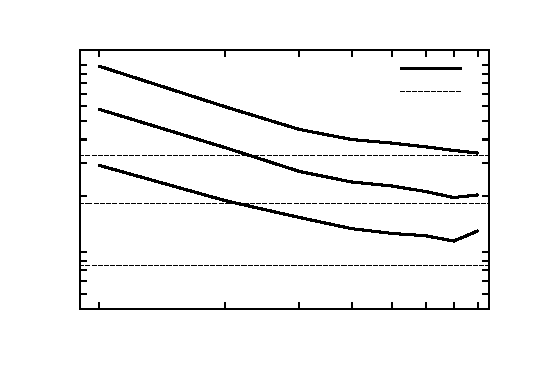
\includegraphics{data/canny/tesla-1024}}%
    \gplfronttext
  \end{picture}%
\endgroup

\vspace{0.5ex}
\caption{Sobel and Canny runtimes, 100 iterations}
\label{fig:SobelAndCannyRuntime}
\end{figure}


% -----------------------------------------------------------------------------
\subsection{Edge Detection}
Figure \ref{fig:CannyExample} shows the result of applying the Canny algorithm to an example image, with our implementation using two thresholds for edge linking hysteresis. Our implementation is broken into several stages: 1) convert the input RGB image to greyscale;  2) perform a Gaussian blur to suppress high frequency noise; 3) differentiate the image with $Sobel_{X,Y}$; 4) compute magnitude and orientation of the vector gradient; 5) classify local maxima of the gradient into strong and weak edges using the thresholds; 6) select points marked as strong edges; 7) link weak edges that are attached to strong edges. The output consists of all points marked as strong edges, as well as any weak edges that are attached to strong edges. A breakdown of runtimes for each of these stages applied to a 1024x1024 image is shown in Figure \ref{fig:CannyBreakdown}, while other sizes are also in Figure \ref{fig:SobelAndCannyRuntime}.

When all is said and done our single threaded implementation is about 4 times slower than OpenCV. With 8 threads it's about 50\% slower with a 512x512 image, 10\% slower for 768x768, and on par for 1024x1024. We feel this is a good result considering that the blur and differentiation stages for the OpenCV version use SIMD operations that we cannot access from Haskell. The OpenCV implementation also uses different data formats for the various stages, converting between 8-bit unsigned and 16-bit signed integers during the application of $Sobel_{X,Y}$. The other stages are performed in a mixture of 8 and 16 bit integer formats. In our own code we also perform the greyscale conversion and edge linking with 8 bit integers. However, using integer operations for the other stages does not help us due to the lack of registers and the aliasing issues mentioned in \S\ref{sec:FillingTheArray}. 

The OpenCV implementation also hand-fuses the ``local maxima'' and ``select strong'' stages, recording an array of indices for strong edges pixels while computing the local maxima. To duplicate this behaviour we would need to provide a joint @mapFilter@ operation, with a corresponding version of @fillCursoredBlock2@. The delayed array approach cannot recover this form of fusion automatically as it cannot be expressed by simple function composition. 

On the positive side, the performance of our Haskell code is more than adequate for real-time edge detection of a video stream. We have an OSX demo available from the Repa homepage \cite{RepaHomePage}. 


% ------------------------------------- FIG
\begin{figure}
\begin{center}
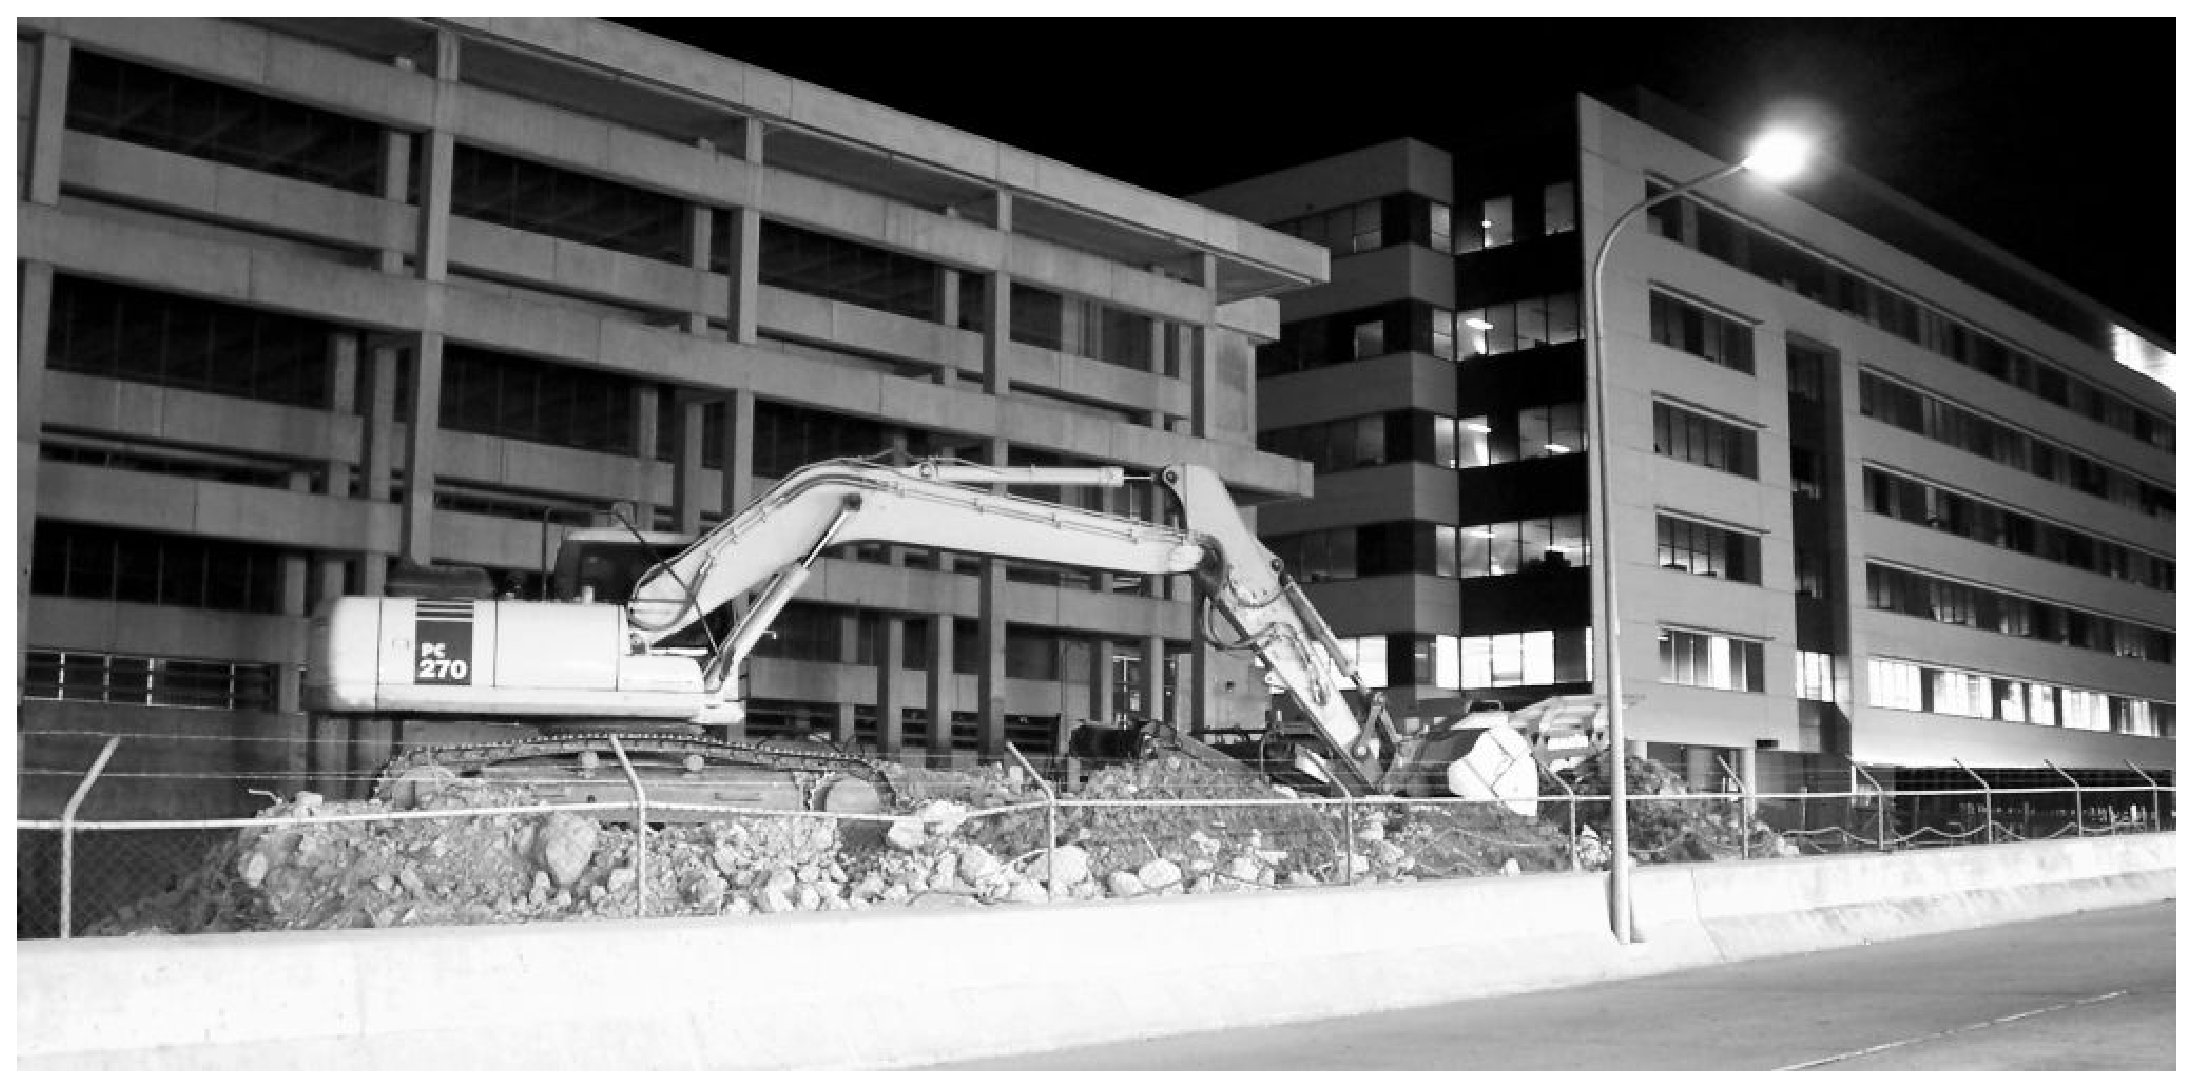
\includegraphics[scale=0.2]{figs/digger-grey-qual80.eps}
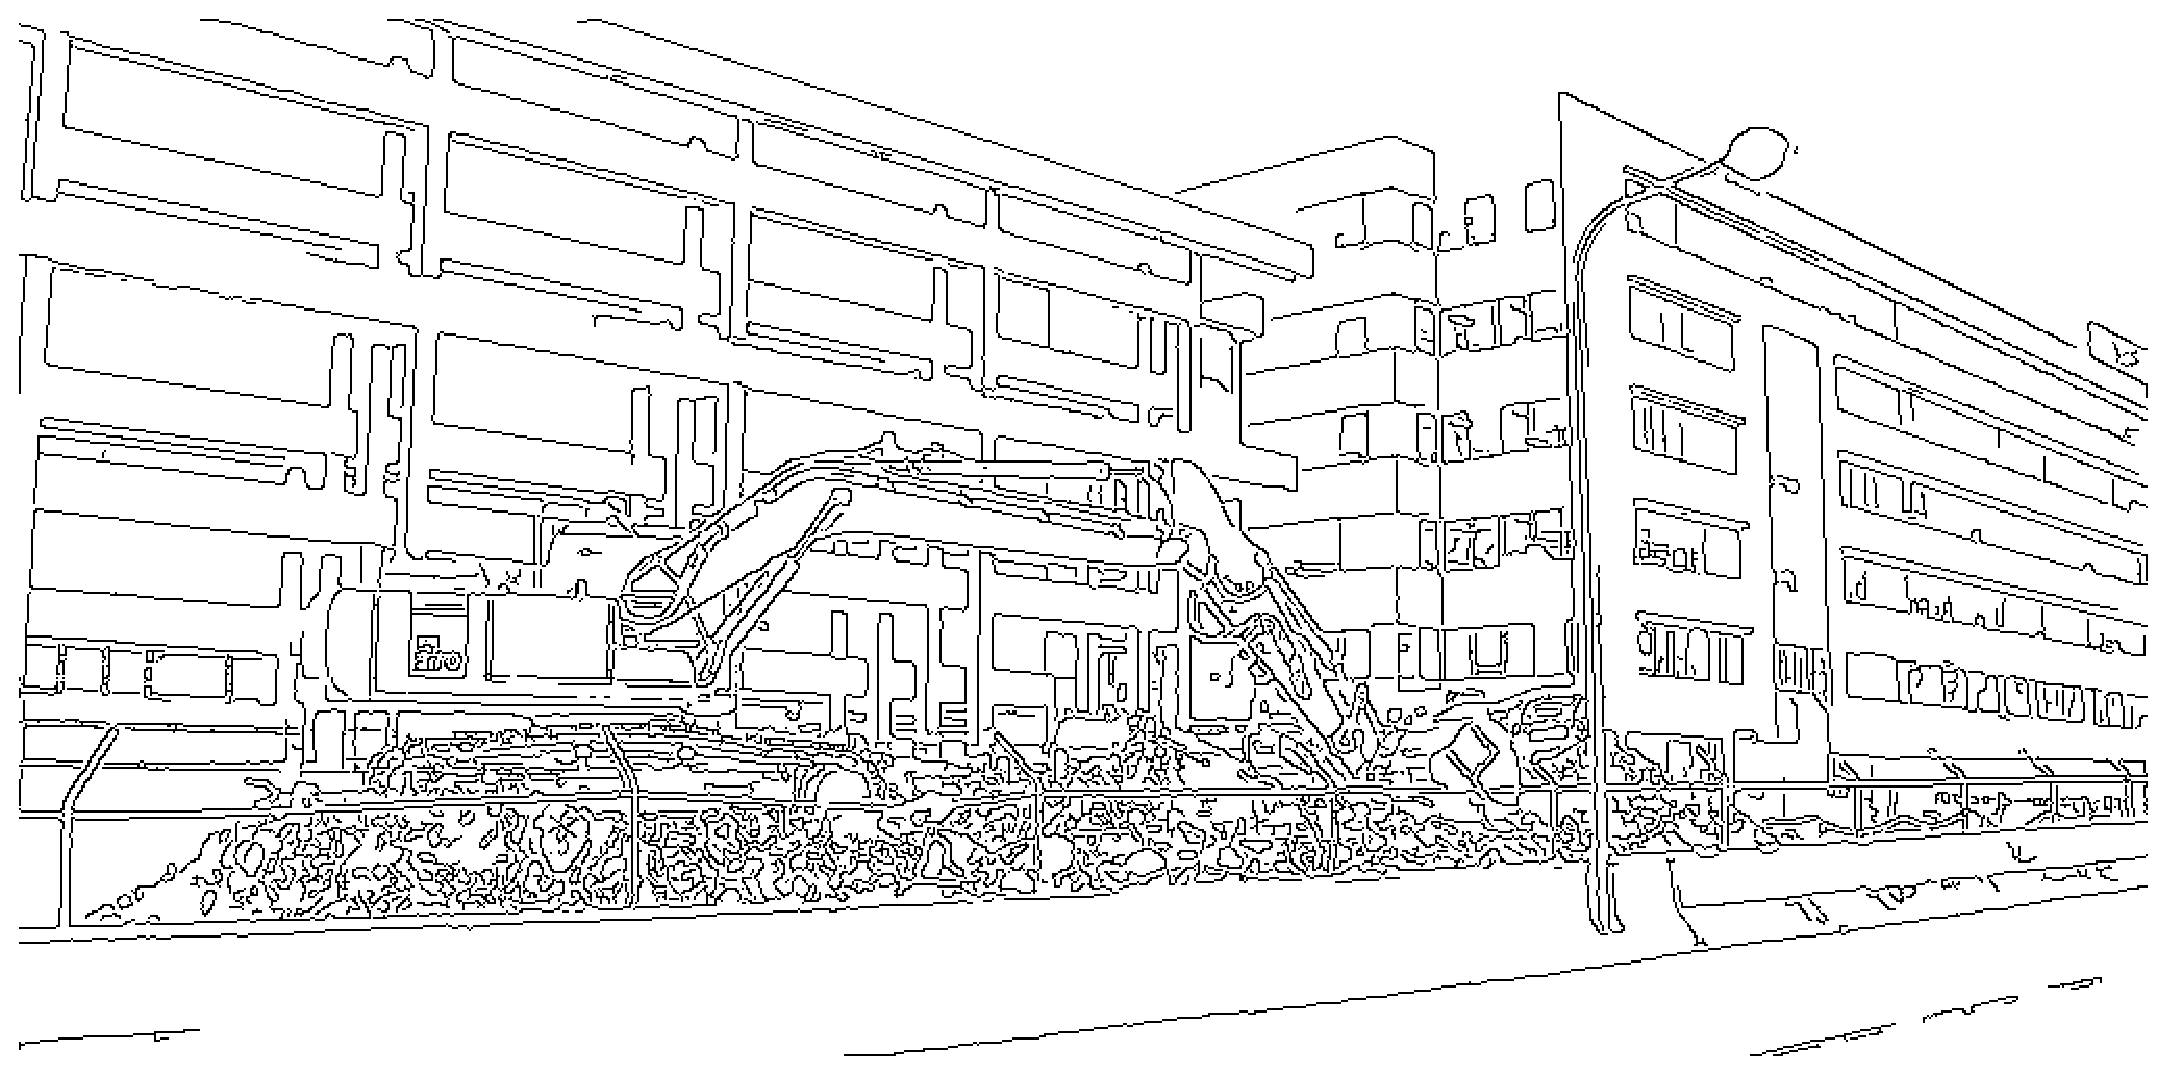
\includegraphics[scale=0.2]{figs/digger-edges.eps}
\vspace{-0.5em}
\end{center}
\caption{Application of Canny edge detector to an image}
\label{fig:CannyExample}
\end{figure}


% ------------------------------------- FIG
\begin{figure}
\vspace{-0.8em}
\hspace{-0.5em}
\begin{tabular}{l|r|rrrr}
		& GCC 4.4.3	& \multicolumn{4}{c}{GHC 7.0.2 + Repa with \# threads} \\
		& OpenCV	&  1     &      2 &      4 &      8	\\
\hline
Grey scale	&  10.59	&  12.05 &   6.19 &   3.25 &   2.08	\\
Gaussian blur	&   3.53	&  17.42 &   9.70 &   5.92 &   5.15	\\
Detect		&  18.95	&  68.73 &  43.81 &  31.21 &  28.49	\\
\hline
~~Differentiate &  fused	&  11.90 &   7.41 &   5.38 &   5.22	\\
~~Mag / Orient 	&  fused	&  27.09 &  16.11 &  10.45 &   7.85	\\
~~Maxima 	&  fused	&  12.87 &   7.84 &   4.83 &   3.32	\\
~~Select strong	&  fused	&  10.01 &   5.68 &   3.60 &   5.16	\\
~~Link edges	&  fused	&  6.86 &   6.77 &   6.95 &   6.94	\\[0.5ex]
\hline
TOTAL (ms)	& 33.05		&  98.25 &  59.70 &  40.38 &  35.72
\end{tabular}

\caption{Canny edge detection, 1024x1024 image}
\label{fig:CannyBreakdown}
\end{figure}


